\section{Performance Evaluation}
\label{sec:Performance}

We conducted our tests in two different mode: scan mode, and monitor mode. In scan mode, the relevant portion of the filesystem is scanned and a tree is built of modification times, both locally and on the server.  The server then sends this information down to the local device, where they are compared to determine what needs to be synchronized. In monitor mode, we use filesystem monitors to watch for changed files on both server and client side, so the only files that are considered for synchronization are those which changed. 

%more info is needed here on how the tests were actually carried out

\subsection{Testing Plan}
In our experiments, we ran the \teledroid application on the background. In turn, we updated multiple files, totaling 1MB in size, on both the local device and the server side three times. In the experiment, we captured CPU and memory usage every 10 seconds. After \teledroid completed one round of file transfers, we recorded the time spent. The experiments were done in both scan mode and monitor mode.
			
\subsection{Hardware Configuration}
Our test device is an Android Dev Phone 1. It has a 528MHZ Qualcomm 7210 processor and 192 MB RAM. It features a touch screen and a trackball for navigation, and provides QWERTY slider keyboard for input. Wi-Fi, GPS, and Bluetooth v2.0 are also present. It also supports 3G WCDMA in 1700/2100 MHz and Quad-band GSM in 850/900/1800/1900 MHz. Note that the Android Dev Phone 1 includes 1GB MicroSC card as an external storage device. It can be replaced with a card of up to 16GB. Concerning the network environment, our tests utilized the University of San Francisco's internet connection, accessed through 802.11g.

\subsection{Results}
The results of our CPU usage tests are shown in Figure~\ref{fig:cpu}. However they were not as we expected. Monitor mode didn't gain any significant advantage over scan mode here. However, synchronization finished faster than in scan mode, so overall cpu usage should be lower than our tests indicate.

\begin{figure}%[htp]
\centering
\subfigure[CPU Usage in Monitor Mode]{\label{fig:cpu-monitor}
    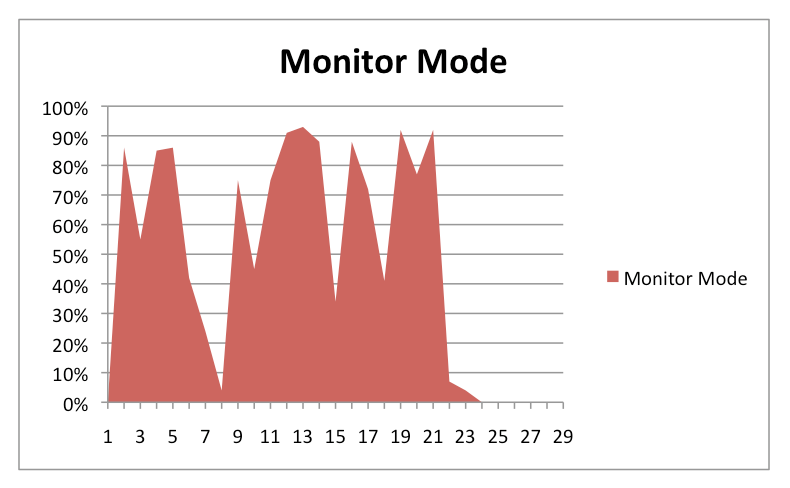
\includegraphics[scale=0.5]{cpu_monitor}}
\hspace{0.20in}
\subfigure[CPU Usage in Scan Mode]{\label{fig:cpu-scan}
	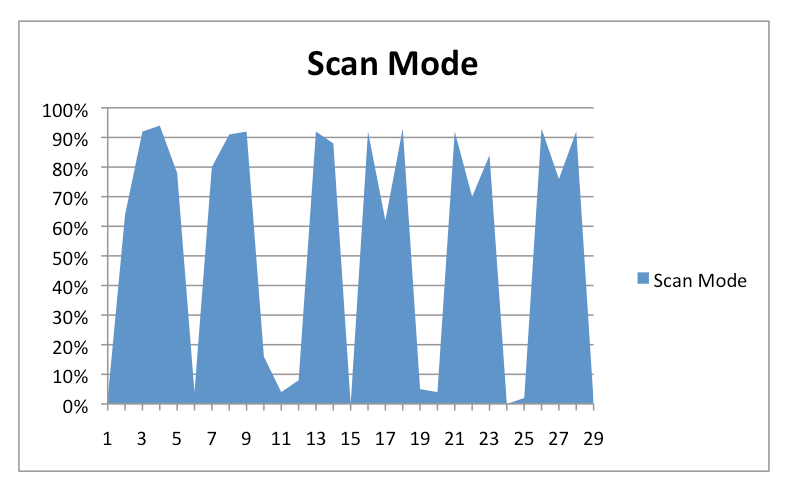
\includegraphics[scale=0.5]{cpu_scan}}
\subfigure[Comparison of CPU Usage]{\label{fig:cpu-comp}
    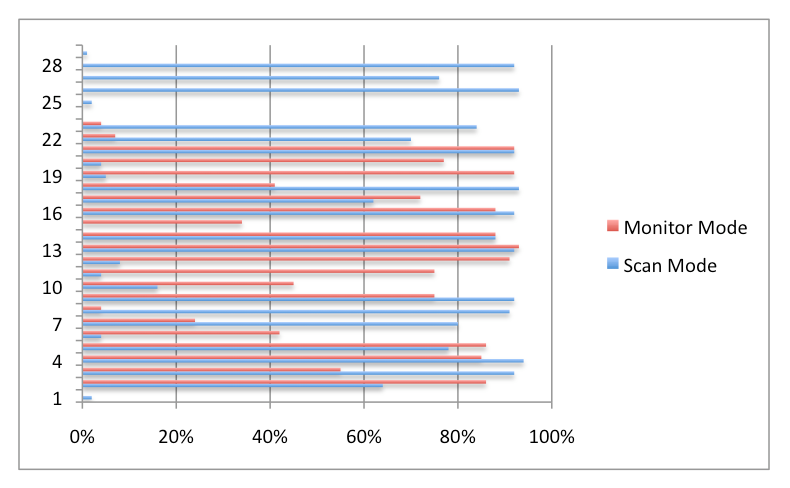
\includegraphics[scale=0.7]{cpu}}
\caption{The CPU usage comparison of Monitor and Scan mode}
\label{fig:cpu}
\end{figure}

Similar to our CPU usage results, the memory usage data was also disappointing. As shown in Figure~\ref{fig:memory}, the memory usage in monitor mode is even higher than scan mode initially. We think this is due in part to the fact that in monitor mode we have to perform an initial complete scan before we can switch over to the low overhead scan mode.  This, combined with the fact that monitor mode makes use of several more threads and an external JNI module seems to explain the difference.

\begin{figure}%[htp]
\centering
\subfigure[Memory Usage in Monitor Mode]{\label{fig:memory-monitor}
    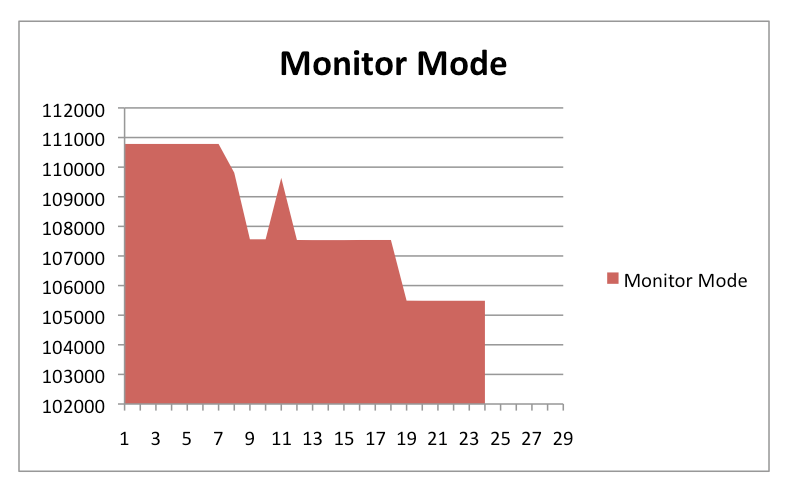
\includegraphics[scale=0.5]{memory_monitor}}
\hspace{0.20in}
\subfigure[Memory Usage in Scan Mode]{\label{fig:memory-scan}
	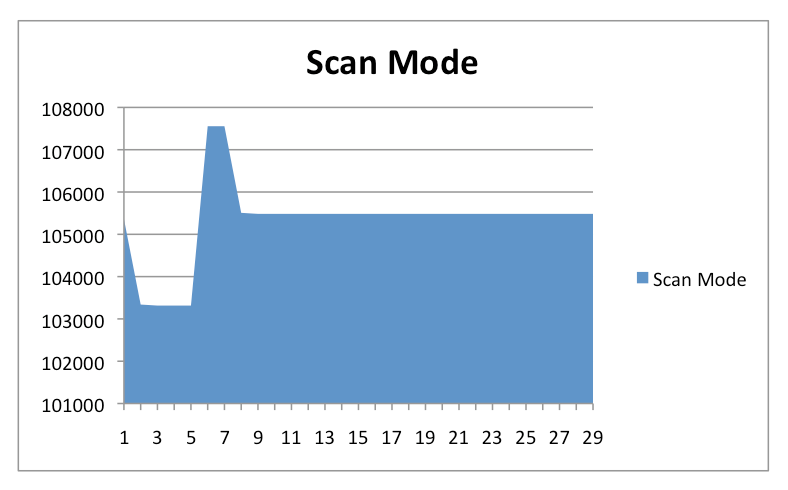
\includegraphics[scale=0.5]{memory_scan}}
\subfigure[Comparison of Memory Usage]{\label{fig:memory-comp}
    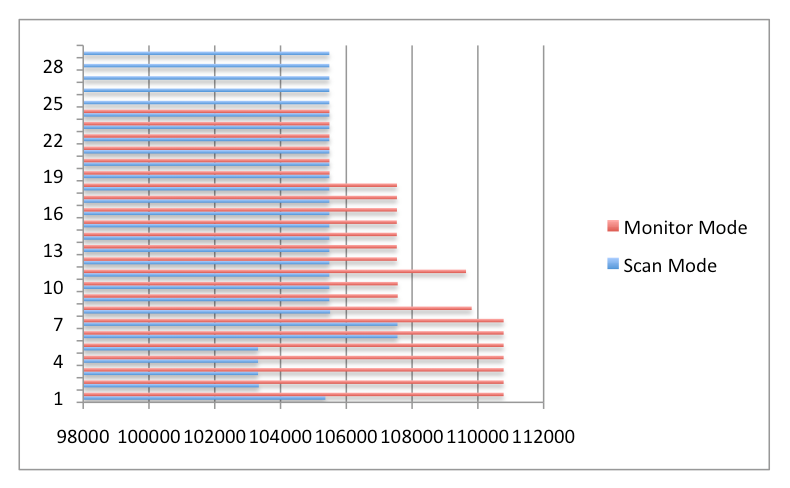
\includegraphics[scale=0.7]{memory}}
\caption{The Memory usage comparison of Monitor and Scan mode}
\label{fig:memory}
\end{figure}

In our tests of synchronization speed we finally got data that indicate that monitor version performs better. 
As we can see in Figure~\ref{fig:speed}, the speed of monitor mode is faster than scan mode on the client side. However, the 
server didn't show significant differences. This may be due to our current server side script using a pull-sync instead of push-sync as client side. 
\begin{figure}[htp]
\centering
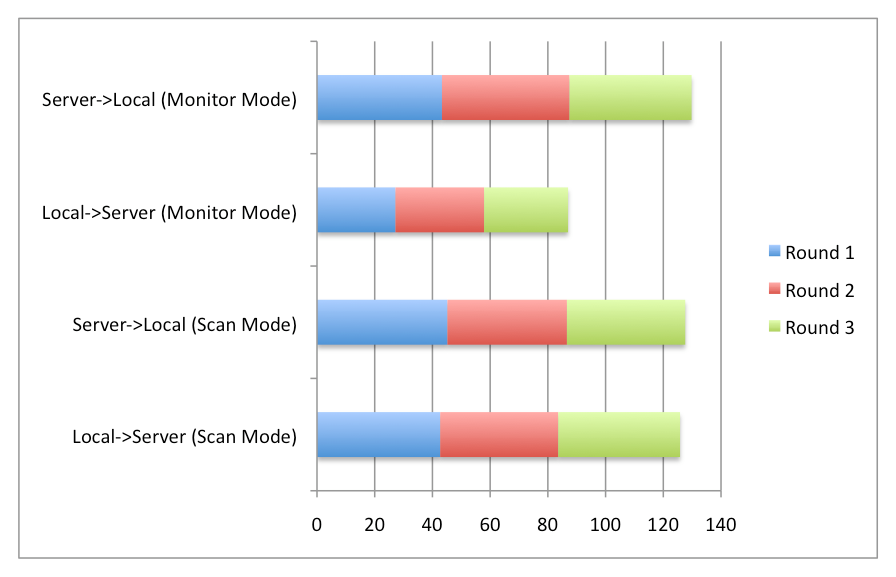
\includegraphics[scale=0.7]{speed}
\caption{Comparison of Synchronization Speed}\label{fig:speed}
\end{figure}
